\documentclass[a4paper,11pt]{article}

%% -------------------------------------------------------
%%  Packages
%% -------------------------------------------------------
\usepackage[T1]{fontenc}
\usepackage[utf8]{inputenc}
\usepackage[english]{babel}
\usepackage{amsmath,amssymb}
\usepackage{booktabs}
\usepackage{siunitx}
\usepackage{geometry}
\usepackage{graphicx}
\usepackage{tikz}
\usepackage{hyperref}
\usepackage{xcolor}
\usepackage{caption}
\usepackage{float}

\geometry{margin=25mm}

\sisetup{
  output-decimal-marker = {.},
  group-separator       = {\,},
  per-mode              = symbol
}

\hypersetup{
  colorlinks = true,
  linkcolor  = blue!60!black,
  urlcolor   = blue!60!black
}

%% -------------------------------------------------------
%%  Title
%% -------------------------------------------------------
\title{\textbf{Thermal Impedance Calculation:\\
Aluminium Plate with Liquid Cooling}}
\author{Davide}
\date{\today}

%% -------------------------------------------------------
\begin{document}
\maketitle
\tableofcontents
\bigskip

%% =======================================================
\section{Introduction and Physical Model}
%% =======================================================

The thermal impedance $Z_{\mathrm{th}}$ (or, in steady-state conditions, the thermal
resistance $R_{\mathrm{th}}$) quantifies the temperature rise per unit of dissipated
power along a thermal path. For a linear, steady-state system:

\begin{equation}
  \Delta T = R_{\mathrm{th}}\, P
  \qquad\left[\si{K/W}\right]
\end{equation}

where $\Delta T$ is the temperature difference between the heat source and the
coolant reference, and $P$ is the dissipated power in watts.

The system under analysis consists of:
\begin{enumerate}
  \item an \textbf{aluminium plate} with dimensions
        $\SI{40}{mm}\times\SI{160}{mm}\times\SI{5}{mm}$
        (the \SI{5}{mm} thickness is along the vertical heat-flow axis);
  \item a \textbf{30\,\% ethylene-glycol/water mixture} flowing along the lower
        face of the plate, with a volumetric flow rate
        $\dot{V}=\SI{24}{l/min}$ through a rectangular channel of height
        $h_c = \SI{12}{mm}$ and width $w_c = \SI{40}{mm}$.
\end{enumerate}

Heat flows vertically from the top surface (source) to the coolant (bottom).
The total thermal resistance is the series combination of two contributions:

\begin{equation}
  \boxed{R_{\mathrm{th,tot}} = R_{\mathrm{cond}} + R_{\mathrm{conv}}}
\end{equation}

The electro-thermal analogy is illustrated in Figure~\ref{fig:circuit}: temperature
plays the role of voltage, power is the current source, and thermal resistance
is the electrical resistance.

\begin{figure}[H]
\centering
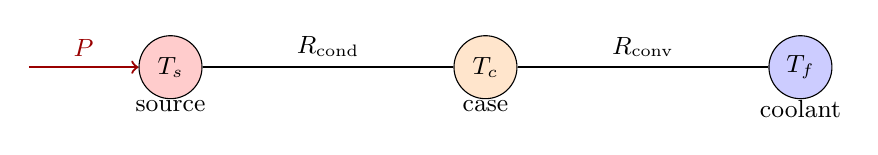
\begin{tikzpicture}[font=\small]
  \node[circle, fill=red!20, draw, minimum size=8mm] (Ts) at (0,0) {$T_s$};
  \node[circle, fill=orange!20, draw, minimum size=8mm] (Tc) at (4,0) {$T_c$};
  \node[circle, fill=blue!20, draw, minimum size=8mm] (Tf) at (8,0) {$T_f$};
  \draw[thick] (Ts) -- node[above]{$R_{\mathrm{cond}}$} (Tc);
  \draw[thick] (Tc) -- node[above]{$R_{\mathrm{conv}}$} (Tf);
  \draw[->, thick, red!60!black] (-1.8,0) -- node[above]{$P$} (Ts);
  \node[below=3mm] at (Ts) {source};
  \node[below=3mm] at (Tc) {case};
  \node[below=3mm] at (Tf) {coolant};
\end{tikzpicture}
\caption{Equivalent electro-thermal circuit. $T_s$ = source temperature,
         $T_c$ = temperature at the bottom face of the aluminium plate,
         $T_f$ = bulk coolant temperature.}
\label{fig:circuit}
\end{figure}

%% =======================================================
\section{Geometry and Input Data}
%% =======================================================

\begin{table}[H]
\centering
\caption{Plate and channel geometry.}
\begin{tabular}{llll}
\toprule
Symbol & Quantity & Value & Unit \\
\midrule
$L$    & Plate length (flow direction)    & 160  & \si{mm} \\
$W$    & Plate width                      & 40   & \si{mm} \\
$t$    & Plate thickness (heat-flow axis) & 5    & \si{mm} \\
$A$    & Active surface area ($L\times W$) & 64  & \si{cm^2} \\
$h_c$  & Channel height                   & 12   & \si{mm} \\
$w_c$  & Channel width                    & 40   & \si{mm} \\
$\dot{V}$ & Volumetric flow rate          & 24   & \si{l/min} \\
\bottomrule
\end{tabular}
\end{table}

The active surface area:
\begin{equation}
  A = L \times W = \SI{0.160}{m} \times \SI{0.040}{m} = \SI{6.4e-3}{m^2}
\end{equation}

%% =======================================================
\section{Conduction Thermal Resistance}
%% =======================================================

Steady-state heat conduction through a plane wall is governed by Fourier's law:

\begin{equation}
  q = -k \frac{\mathrm{d}T}{\mathrm{d}z}
\end{equation}

where $q\,[\si{W/m^2}]$ is the heat flux and $k\,[\si{W/(m\cdot K)}]$ is the
thermal conductivity. For a flat wall of thickness $t$, area $A$, and total power
$P = q\cdot A$, the conduction thermal resistance is:

\begin{equation}
  \boxed{R_{\mathrm{cond}} = \frac{t}{k\,A}}
  \qquad \left[\si{K/W}\right]
\end{equation}

For general-purpose aluminium (6xxx series):
$k_{\mathrm{Al}} = \SI{160}{W/(m\cdot K)}$.

\begin{equation}
  R_{\mathrm{cond}} = \frac{\SI{5e-3}{m}}{\SI{160}{W/(m\cdot K)} \times \SI{6.4e-3}{m^2}}
  = \SI{4.88e-3}{K/W} \approx \SI{4.88}{mK/W}
\end{equation}

\noindent\textbf{Note:} this value is small compared to the convective resistance,
confirming that the aluminium plate is not the thermal bottleneck in this geometry.

%% =======================================================
\section{Convection Thermal Resistance}
%% =======================================================

\subsection{Fluid Properties}

The coolant is a 30\,\% ethylene-glycol/water mixture.
Thermo-physical properties at a representative operating temperature of
$\approx\SI{50}{\celsius}$ are listed in Table~\ref{tab:fluid}.

\begin{table}[H]
\centering
\caption{Thermo-physical properties of EG\,30\,\% (vol.) at $T\approx\SI{50}{\celsius}$.}
\label{tab:fluid}
\begin{tabular}{llll}
\toprule
Symbol & Property & Value & Unit \\
\midrule
$\rho$  & Density               & 1040  & \si{kg/m^3}        \\
$c_p$   & Specific heat         & 3800  & \si{J/(kg\cdot K)} \\
$\mu$   & Dynamic viscosity     & 0.82  & \si{mPa\cdot s}    \\
$k_f$   & Thermal conductivity  & 0.45  & \si{W/(m\cdot K)}  \\
$\Pr$   & Prandtl number        & 6.92  & --                 \\
\bottomrule
\end{tabular}
\end{table}

The Prandtl number:
\begin{equation}
  \Pr = \frac{\mu\, c_p}{k_f}
      = \frac{\SI{8.2e-4}{Pa\cdot s} \times \SI{3800}{J/(kg\cdot K)}}{\SI{0.45}{W/(m\cdot K)}}
      \approx 6.92
\end{equation}

\subsection{Flow Rate and Mean Velocity}

The volumetric flow rate:
\begin{equation}
  \dot{V} = \SI{24}{l/min} = \frac{24}{60\times 1000}\,\si{m^3/s}
          = \SI{4.0e-4}{m^3/s}
\end{equation}

Cross-sectional area of the channel:
\begin{equation}
  A_c = h_c \times w_c = \SI{12e-3}{m} \times \SI{40e-3}{m} = \SI{4.8e-4}{m^2}
\end{equation}

Mean fluid velocity:
\begin{equation}
  \bar{v} = \frac{\dot{V}}{A_c} = \frac{\SI{4.0e-4}{m^3/s}}{\SI{4.8e-4}{m^2}}
          \approx \SI{0.833}{m/s}
\end{equation}

\subsection{Hydraulic Diameter}

For a rectangular duct with height $h_c$ and width $w_c$:
\begin{equation}
  D_h = \frac{4\,A_c}{P_w} = \frac{4\,h_c\,w_c}{2\,(h_c+w_c)}
      = \frac{4\times\SI{12e-3}{m}\times\SI{40e-3}{m}}{2\,(\SI{12e-3}{m}+\SI{40e-3}{m})}
      \approx \SI{18.46}{mm}
\end{equation}

where $P_w$ is the wetted perimeter.

\subsection{Reynolds Number}

\begin{equation}
  \mathrm{Re} = \frac{\rho\,\bar{v}\,D_h}{\mu}
       = \frac{1040 \times 0.833 \times \SI{18.46e-3}{}}{8.2\times10^{-4}}
       \approx 19\,512
\end{equation}

Since $\mathrm{Re} \gg 4000$, the flow is in the \textbf{fully turbulent regime}.

\subsection{Nusselt Number Correlations}

\subsubsection{Dittus--Boelter Correlation}

For a heated fluid ($n=0.4$), valid for $\mathrm{Re}>10^4$,
$0.7<\Pr<160$, $L/D_h>60$:
\begin{equation}
  \mathrm{Nu}_{\mathrm{DB}} = 0.023\,\mathrm{Re}^{0.8}\,\Pr^{0.4}
                    = 0.023 \times 19512^{0.8} \times 6.92^{0.4}
                    \approx 132.0
\end{equation}

\subsubsection{Gnielinski Correlation (Recommended)}

More accurate over $3000 < \mathrm{Re} < 5\times10^6$, $0.5 < \Pr < 2000$,
using the Petukhov friction factor $f$:

\begin{equation}
  f = \bigl(0.790\ln\mathrm{Re} - 1.64\bigr)^{-2}
    = \bigl(0.790\times\ln 19512 - 1.64\bigr)^{-2}
    \approx 0.02632
\end{equation}

\begin{equation}
  \mathrm{Nu}_{\mathrm{G}} = \frac{(f/8)\,(\mathrm{Re}-1000)\,\Pr}
                         {1 + 12.7\sqrt{f/8}\,(\Pr^{2/3}-1)}
                  = \frac{(0.02632/8)\times 18512 \times 6.92}
                         {1 + 12.7\sqrt{0.02632/8}\,(6.92^{2/3}-1)}
                  \approx 144.5
\end{equation}

\subsection{Convective Coefficient and Resistance}

Using the Gnielinski correlation:
\begin{equation}
  h_{\mathrm{conv}} = \frac{\mathrm{Nu}_{\mathrm{G}}\,k_f}{D_h}
                    = \frac{144.5 \times \SI{0.45}{W/(m\cdot K)}}{\SI{18.46e-3}{m}}
                    \approx \SI{3523}{W/(m^2\cdot K)}
\end{equation}

Convective thermal resistance over the full plate area $A$:
\begin{equation}
  \boxed{R_{\mathrm{conv}} = \frac{1}{h_{\mathrm{conv}}\,A}
                            = \frac{1}{\SI{3523}{W/(m^2\cdot K)}\times\SI{6.4e-3}{m^2}}
                            \approx \SI{44.36}{mK/W}}
\end{equation}

%% =======================================================
\section{Total Thermal Resistance and Results}
%% =======================================================

\begin{equation}
  R_{\mathrm{th,tot}} = R_{\mathrm{cond}} + R_{\mathrm{conv}}
                      = \SI{4.88}{mK/W} + \SI{44.36}{mK/W}
                      \approx \SI{49.24}{mK/W}
\end{equation}

\begin{table}[H]
\centering
\caption{Summary of thermal resistance contributions ($h_c = \SI{12}{mm}$).}
\begin{tabular}{llcc}
\toprule
Contribution & Expression & Value [\si{mK/W}] & \% of total \\
\midrule
Aluminium conduction    & $t/(k_{\mathrm{Al}}\,A)$      &  4.88 &  9.9\% \\
Convection (Gnielinski) & $1/(h_{\mathrm{conv}}\,A)$    & 44.36 & 90.1\% \\
\midrule
\textbf{Total} & $R_{\mathrm{cond}}+R_{\mathrm{conv}}$ & \textbf{49.24} & 100\% \\
\bottomrule
\end{tabular}
\end{table}

The source-to-coolant temperature rise for dissipated power $P$:
\begin{equation}
  \Delta T = R_{\mathrm{th,tot}}\times P
           \approx \SI{49.24e-3}{K/W} \times P
\end{equation}

For example, at $P = \SI{1000}{W}$:
\begin{equation}
  \Delta T \approx \SI{49.24e-3}{K/W} \times \SI{1000}{W} \approx \SI{49.2}{K}
\end{equation}

\noindent\textbf{Comparison with $h_c = \SI{5}{mm}$:} increasing the channel height
from \SI{5}{mm} to \SI{12}{mm} reduces the mean velocity from \SI{2.0}{m/s} to
\SI{0.83}{m/s} and raises $D_h$ from \SI{8.89}{mm} to \SI{18.46}{mm}. Both effects
lower turbulence intensity, causing $h_{\mathrm{conv}}$ to drop from
$\approx\SI{8300}{W/(m^2 K)}$ to $\approx\SI{3500}{W/(m^2 K)}$ and
$R_{\mathrm{th,tot}}$ to more than double (from \SI{23.7}{mK/W} to \SI{49.2}{mK/W}).

%% =======================================================
\section{Dynamic Thermal Impedance (RC Model)}
%% =======================================================

In transient operation, the thermal response is modelled by an equivalent RC network.
For a single lumped thermal mass (the aluminium plate):

\begin{equation}
  C_{\mathrm{th}} = \rho_{\mathrm{Al}}\,c_{p,\mathrm{Al}}\,V_{\mathrm{Al}}
\end{equation}

With $\rho_{\mathrm{Al}} = \SI{2700}{kg/m^3}$,
$c_{p,\mathrm{Al}} = \SI{900}{J/(kg\cdot K)}$,
$V_{\mathrm{Al}} = L\times W\times t = \SI{3.2e-5}{m^3}$:

\begin{equation}
  C_{\mathrm{th}} = 2700 \times 900 \times \SI{3.2e-5}{m^3}
                  \approx \SI{77.8}{J/K}
\end{equation}

The thermal time constant of the conduction path:
\begin{equation}
  \tau = R_{\mathrm{cond}}\times C_{\mathrm{th}}
       = \SI{4.88e-3}{K/W} \times \SI{77.8}{J/K}
       \approx \SI{0.38}{s}
\end{equation}

The thermal impedance in the frequency domain (single-pole Foster model):
\begin{equation}
  Z_{\mathrm{th}}(j\omega) = \frac{R_{\mathrm{th,tot}}}{1 + j\omega\tau}
\end{equation}

For a power pulse of duration $t_p$, the peak temperature rise is estimated from
the transient impedance curve:
\begin{equation}
  \Delta T_{\mathrm{peak}} = Z_{\mathrm{th}}(t_p)\times P_{\mathrm{peak}}
\end{equation}

%% =======================================================
\section{Model Validity and Assumptions}
%% =======================================================

\begin{enumerate}
  \item \textbf{Steady-state analysis.} The calculation provides the static resistance
        $R_{\mathrm{th}}$. For transient analysis a full Foster or Cauer RC network is required.

  \item \textbf{One-dimensional heat flow.} Valid for uniform power distribution.
        Localised sources (e.g.\ IGBT chips) introduce an additional spreading
        resistance.

  \item \textbf{Smooth-wall channel.} The Gnielinski correlation applies to smooth-walled
        ducts. Pin-fin or corrugated structures significantly enhance $h_{\mathrm{conv}}$.

  \item \textbf{Constant fluid properties.} Properties of the glycol mixture vary with
        temperature; a more accurate analysis would iterate on the mean film temperature.

  \item \textbf{Contact resistance.} The interfacial resistance between the aluminium
        plate and the channel wall is not included; it depends on surface roughness and
        any thermal interface material applied.

  \item \textbf{Channel height impact.} A larger $h_c$ increases $D_h$ and reduces
        $\bar{v}$ at constant flow rate, both lowering the Nusselt number and
        increasing $R_{\mathrm{conv}}$. For optimal performance the channel should be
        as shallow as mechanically permissible, or equipped with internal fins.
\end{enumerate}

%% =======================================================
\section{Conclusions}
%% =======================================================

The steady-state total thermal resistance of the aluminium-plate/glycol-cooled
system with channel height $h_c = \SI{12}{mm}$ is:

\begin{equation}
  R_{\mathrm{th,tot}} \approx \SI{49.24}{mK/W}
\end{equation}

Convection dominates (\SI{\approx 90}{\percent} of the total). The \SI{5}{mm}
aluminium layer contributes only \SI{4.88}{mK/W} and is not the limiting factor.
Compared to the shallower $h_c = \SI{5}{mm}$ configuration
($R_{\mathrm{th,tot}}\approx\SI{23.7}{mK/W}$), the deeper channel more than doubles
the total thermal resistance. To improve cooling performance one should reduce the
channel height, increase the flow rate, or introduce pin-fin structures to enhance
convection.

\end{document}
